\documentclass[14pt, fleqn, xcolor={dvipsnames, table}]{beamer}
\usepackage[T2A]{fontenc}
\usepackage[utf8]{inputenc}
\usepackage[english,russian]{babel}
\usepackage{amssymb,amsfonts,amsmath,mathtext}
\usepackage{cite,enumerate,float,indentfirst}
\usepackage{cancel}
\usepackage{color}
\usepackage{hyperref}
\hypersetup{colorlinks,urlcolor=NavyBlue}

\usepackage{tikz}                   
\usetikzlibrary{shadows}

% \usepackage{enumitem}
% \setitemize{label=\usebeamerfont*{itemize item}%
%   \usebeamercolor[fg]{itemize item}
%   \usebeamertemplate{itemize item}}

\graphicspath{{images/}}

\usetheme{Boadilla}
\usecolortheme{seahorse}
\usefonttheme{serif}
\renewcommand{\CancelColor}{\color{red}}

\setbeamercolor{footline}{fg=Blue!50}
\setbeamertemplate{footline}

\title{Автоматическое проектирование кварталов}
\author[]{
    \small{
        Амосов Федор, СПбГУ\\
        Краевский Михаил, СПбГАСУ
    }
}
\date{}

\begin{document}

    \begin{frame}
        \maketitle
        \small
    \end{frame}

    \section{Постановка задачи}  
    
        \begin{frame}{Постановка задачи}
            \begin{center}
                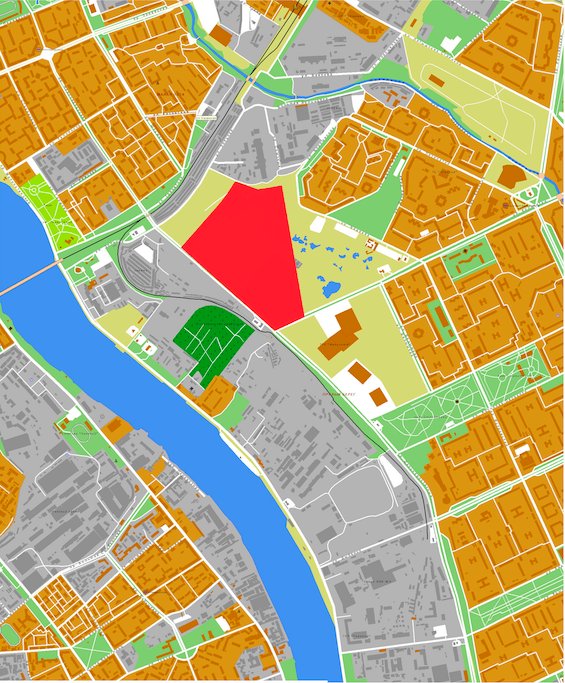
\includegraphics[scale=0.26]{top-plan.png}~
                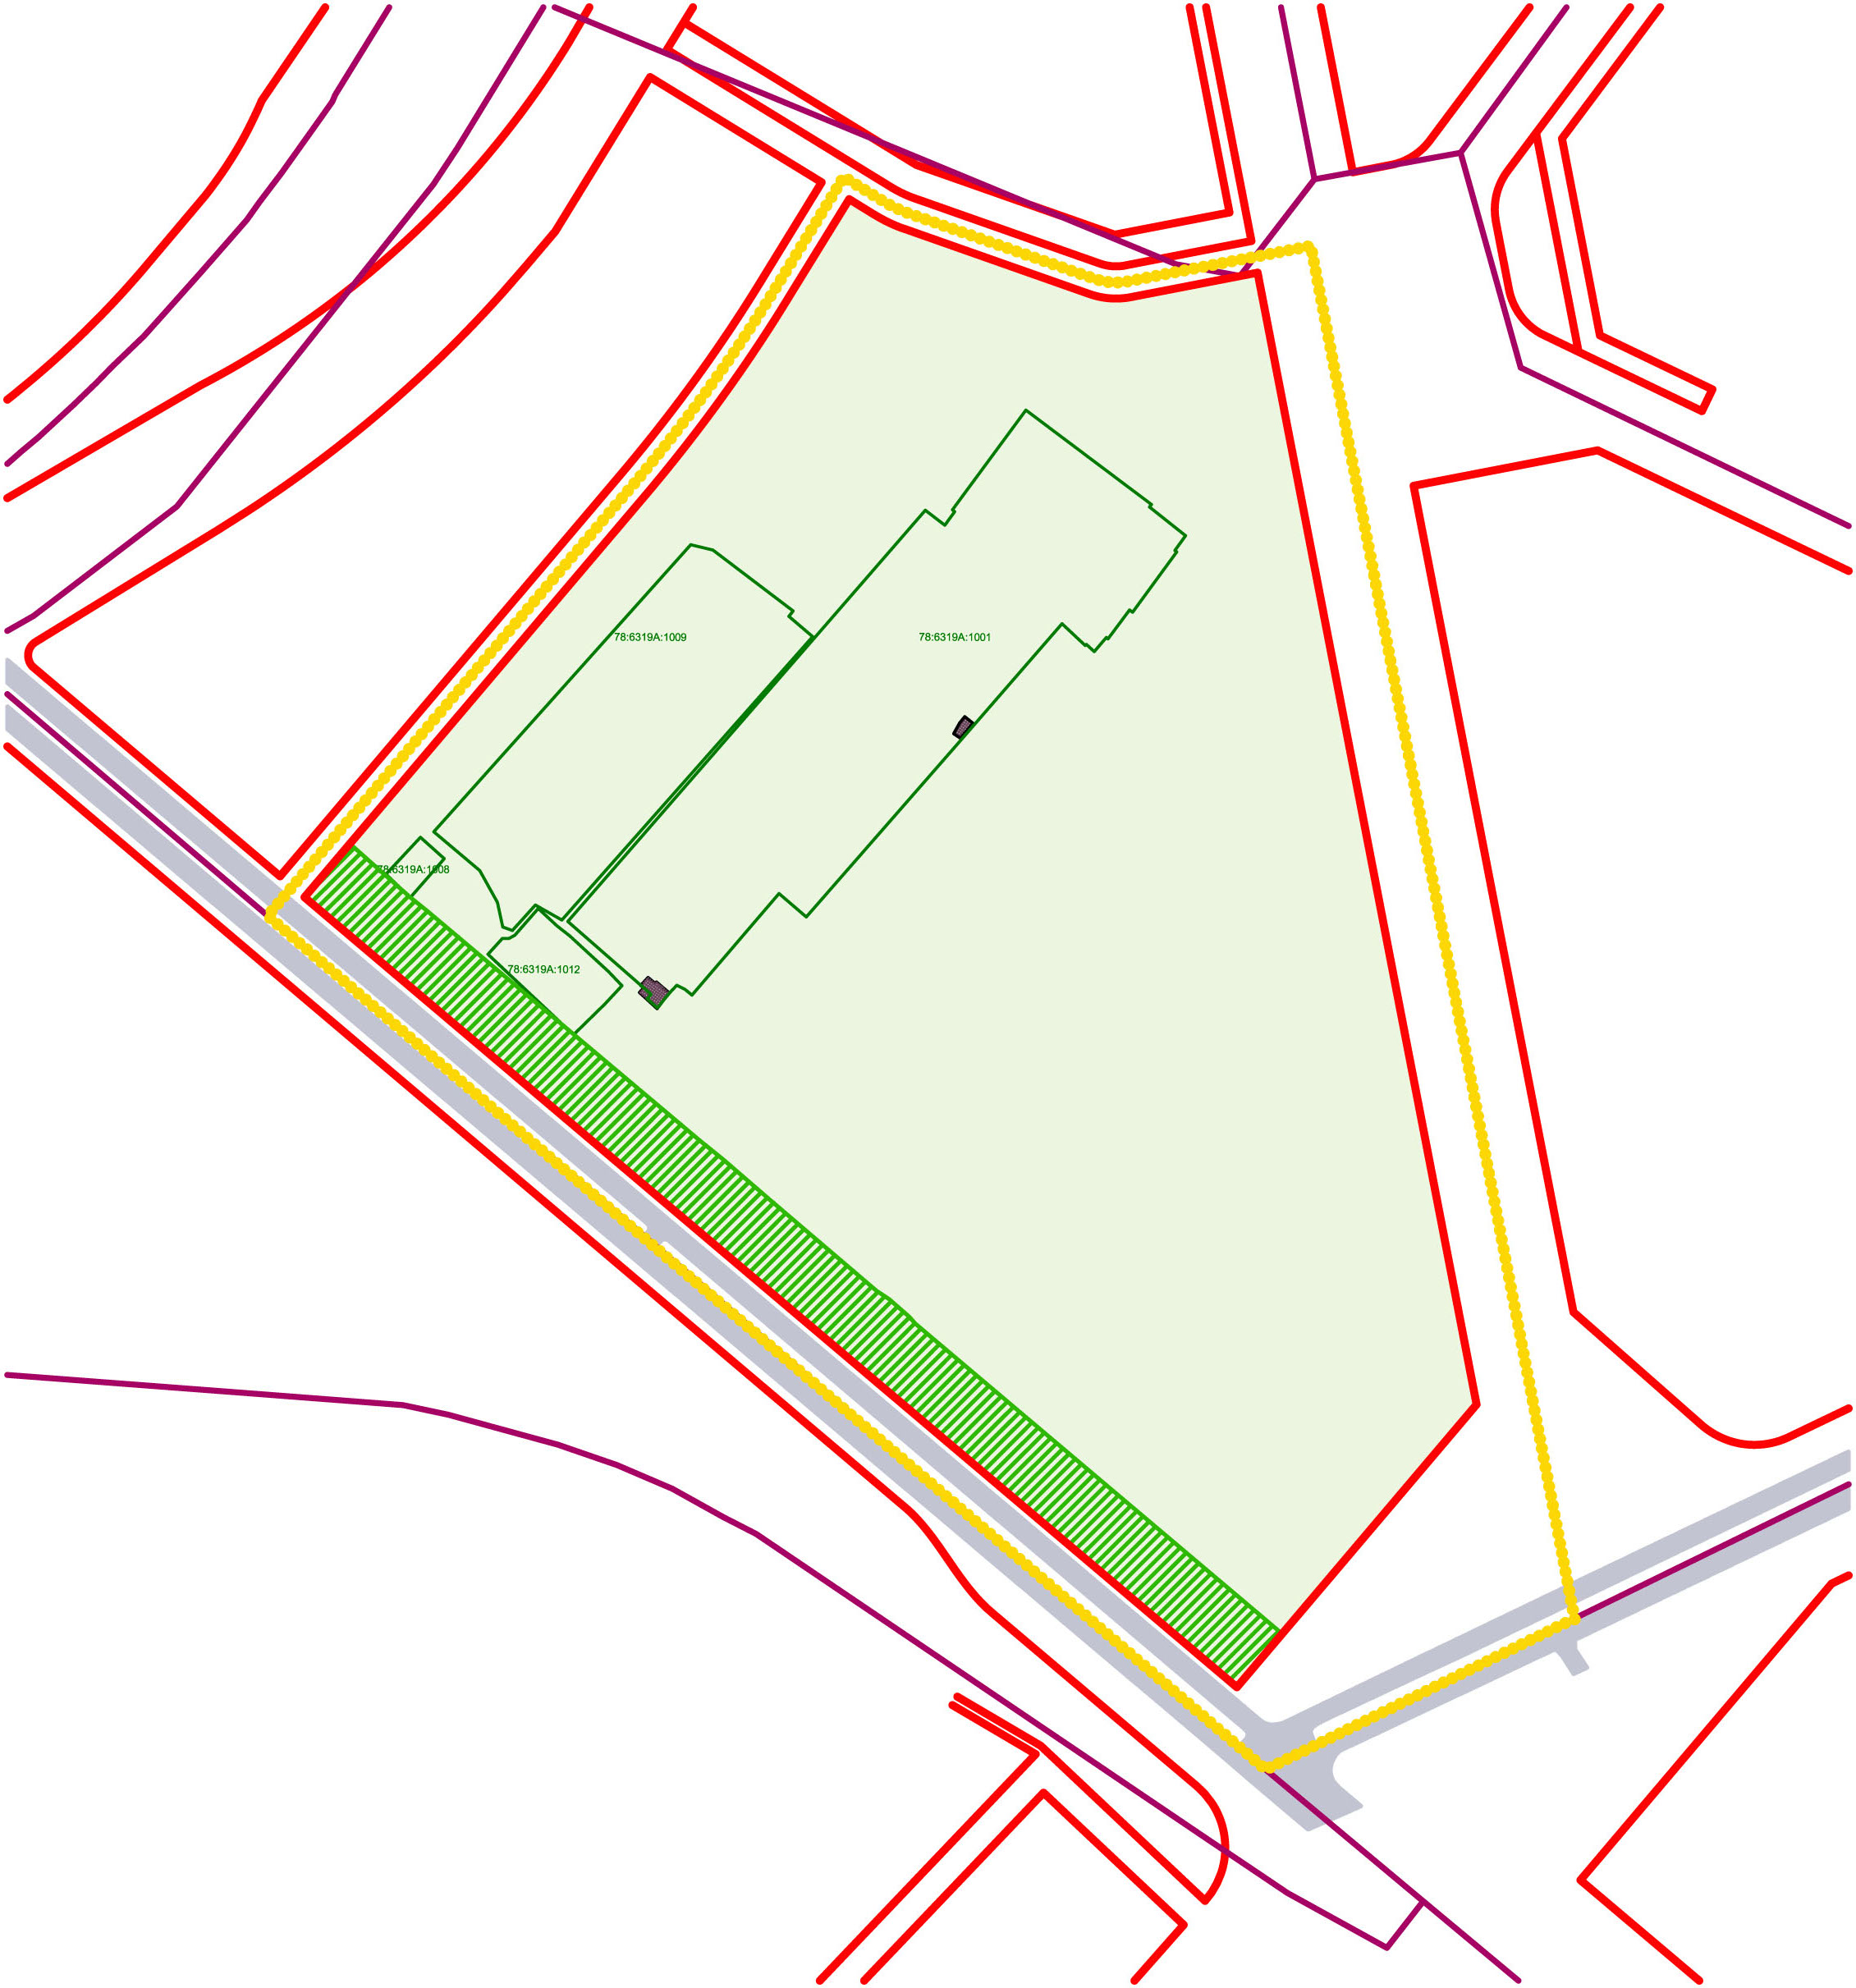
\includegraphics[scale=0.27]{empty.jpg}
            \end{center}                 
        \end{frame}
        
        \begin{frame}{Постановка задачи}
            \begin{center}
                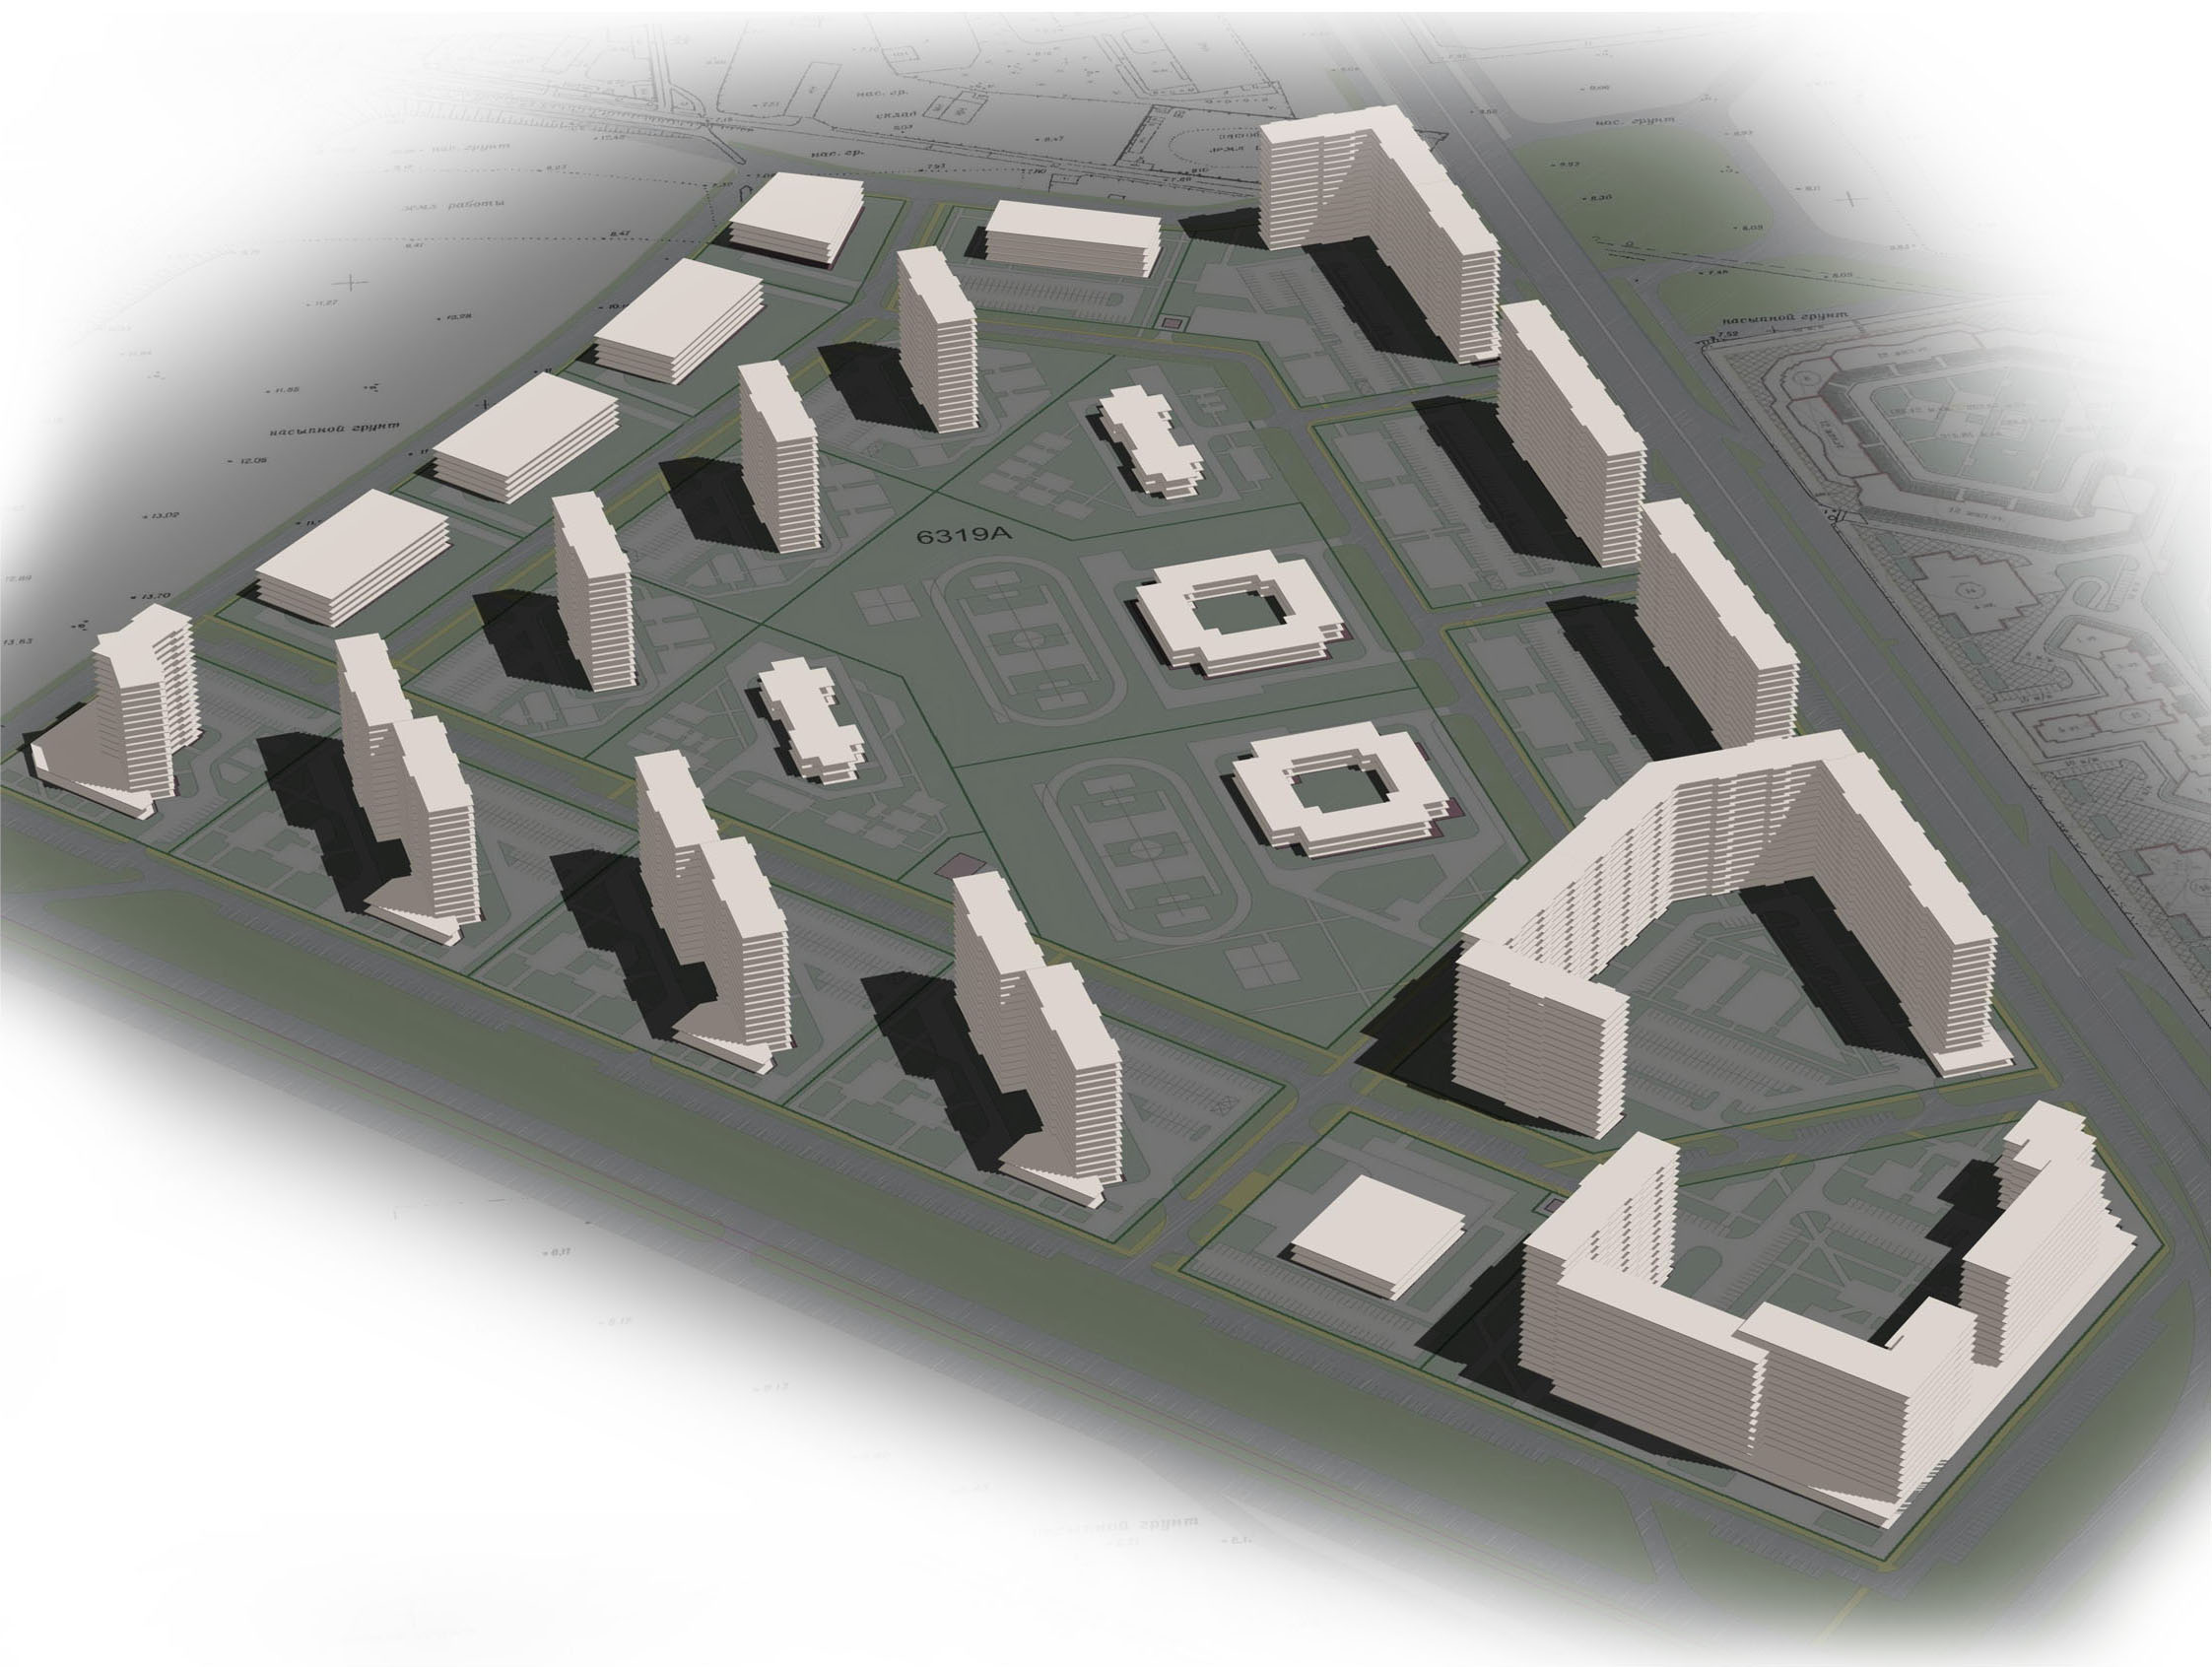
\includegraphics[scale=0.08]{3d.jpg}~
                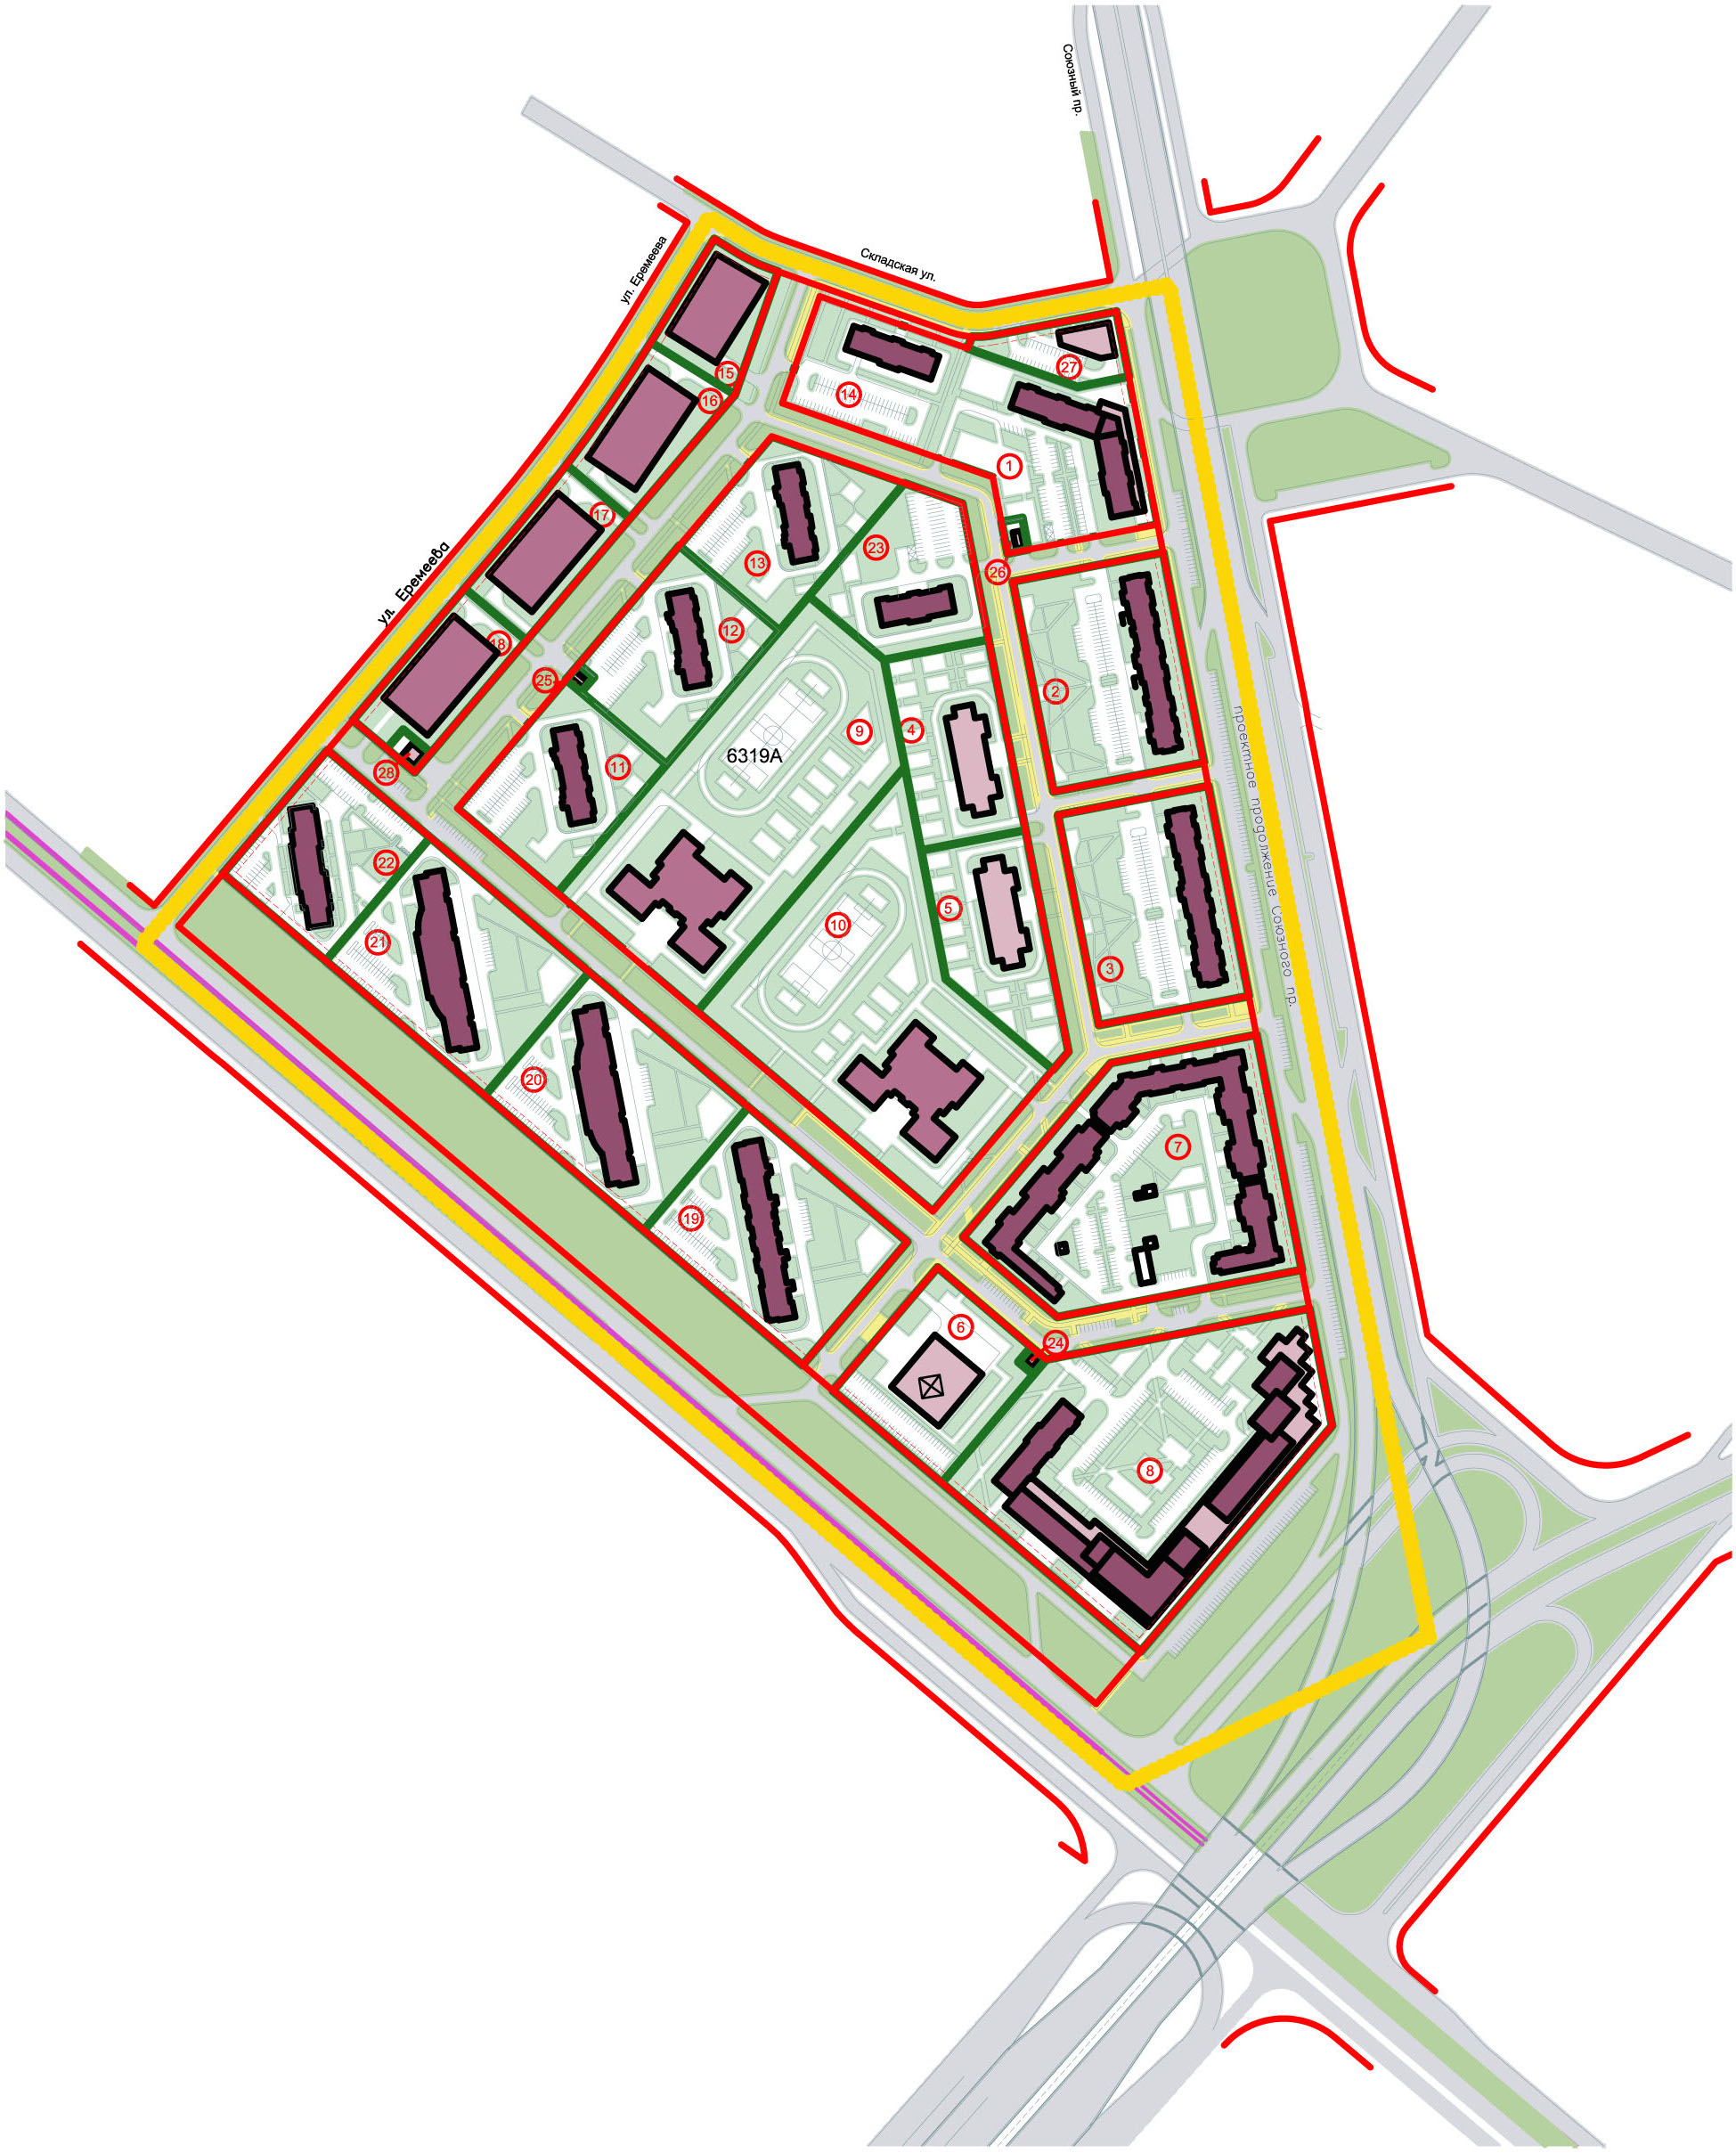
\includegraphics[scale=0.28]{fill.jpg}
            \end{center}                 
        \end{frame}
        
        \begin{frame}{Линейное программирование}
            \begin{itemize}
                \item Площадь квартир $\le$ 2.3 * Площадь квартала
                \item Высота домов $\le$ Max разрешенная высота
                \item Площадь озеленения $\ge$ 0.23 * Площадь квартир
                \item 28 м$^2$ на человека
                \item Вместимость школ $\ge 120$ мест на $1000$ чел.
                \item Вместимость садиков $\ge 55$ мест на $1000$ чел.
                \item Хотя бы одно парковочное место на 80 м$^2$ жилья
                \item ...
            \end{itemize}
            Площадь квартир $\longrightarrow$ max            
                          
        \end{frame}
        
        \begin{frame}{Проблематика}
            \begin{center}
                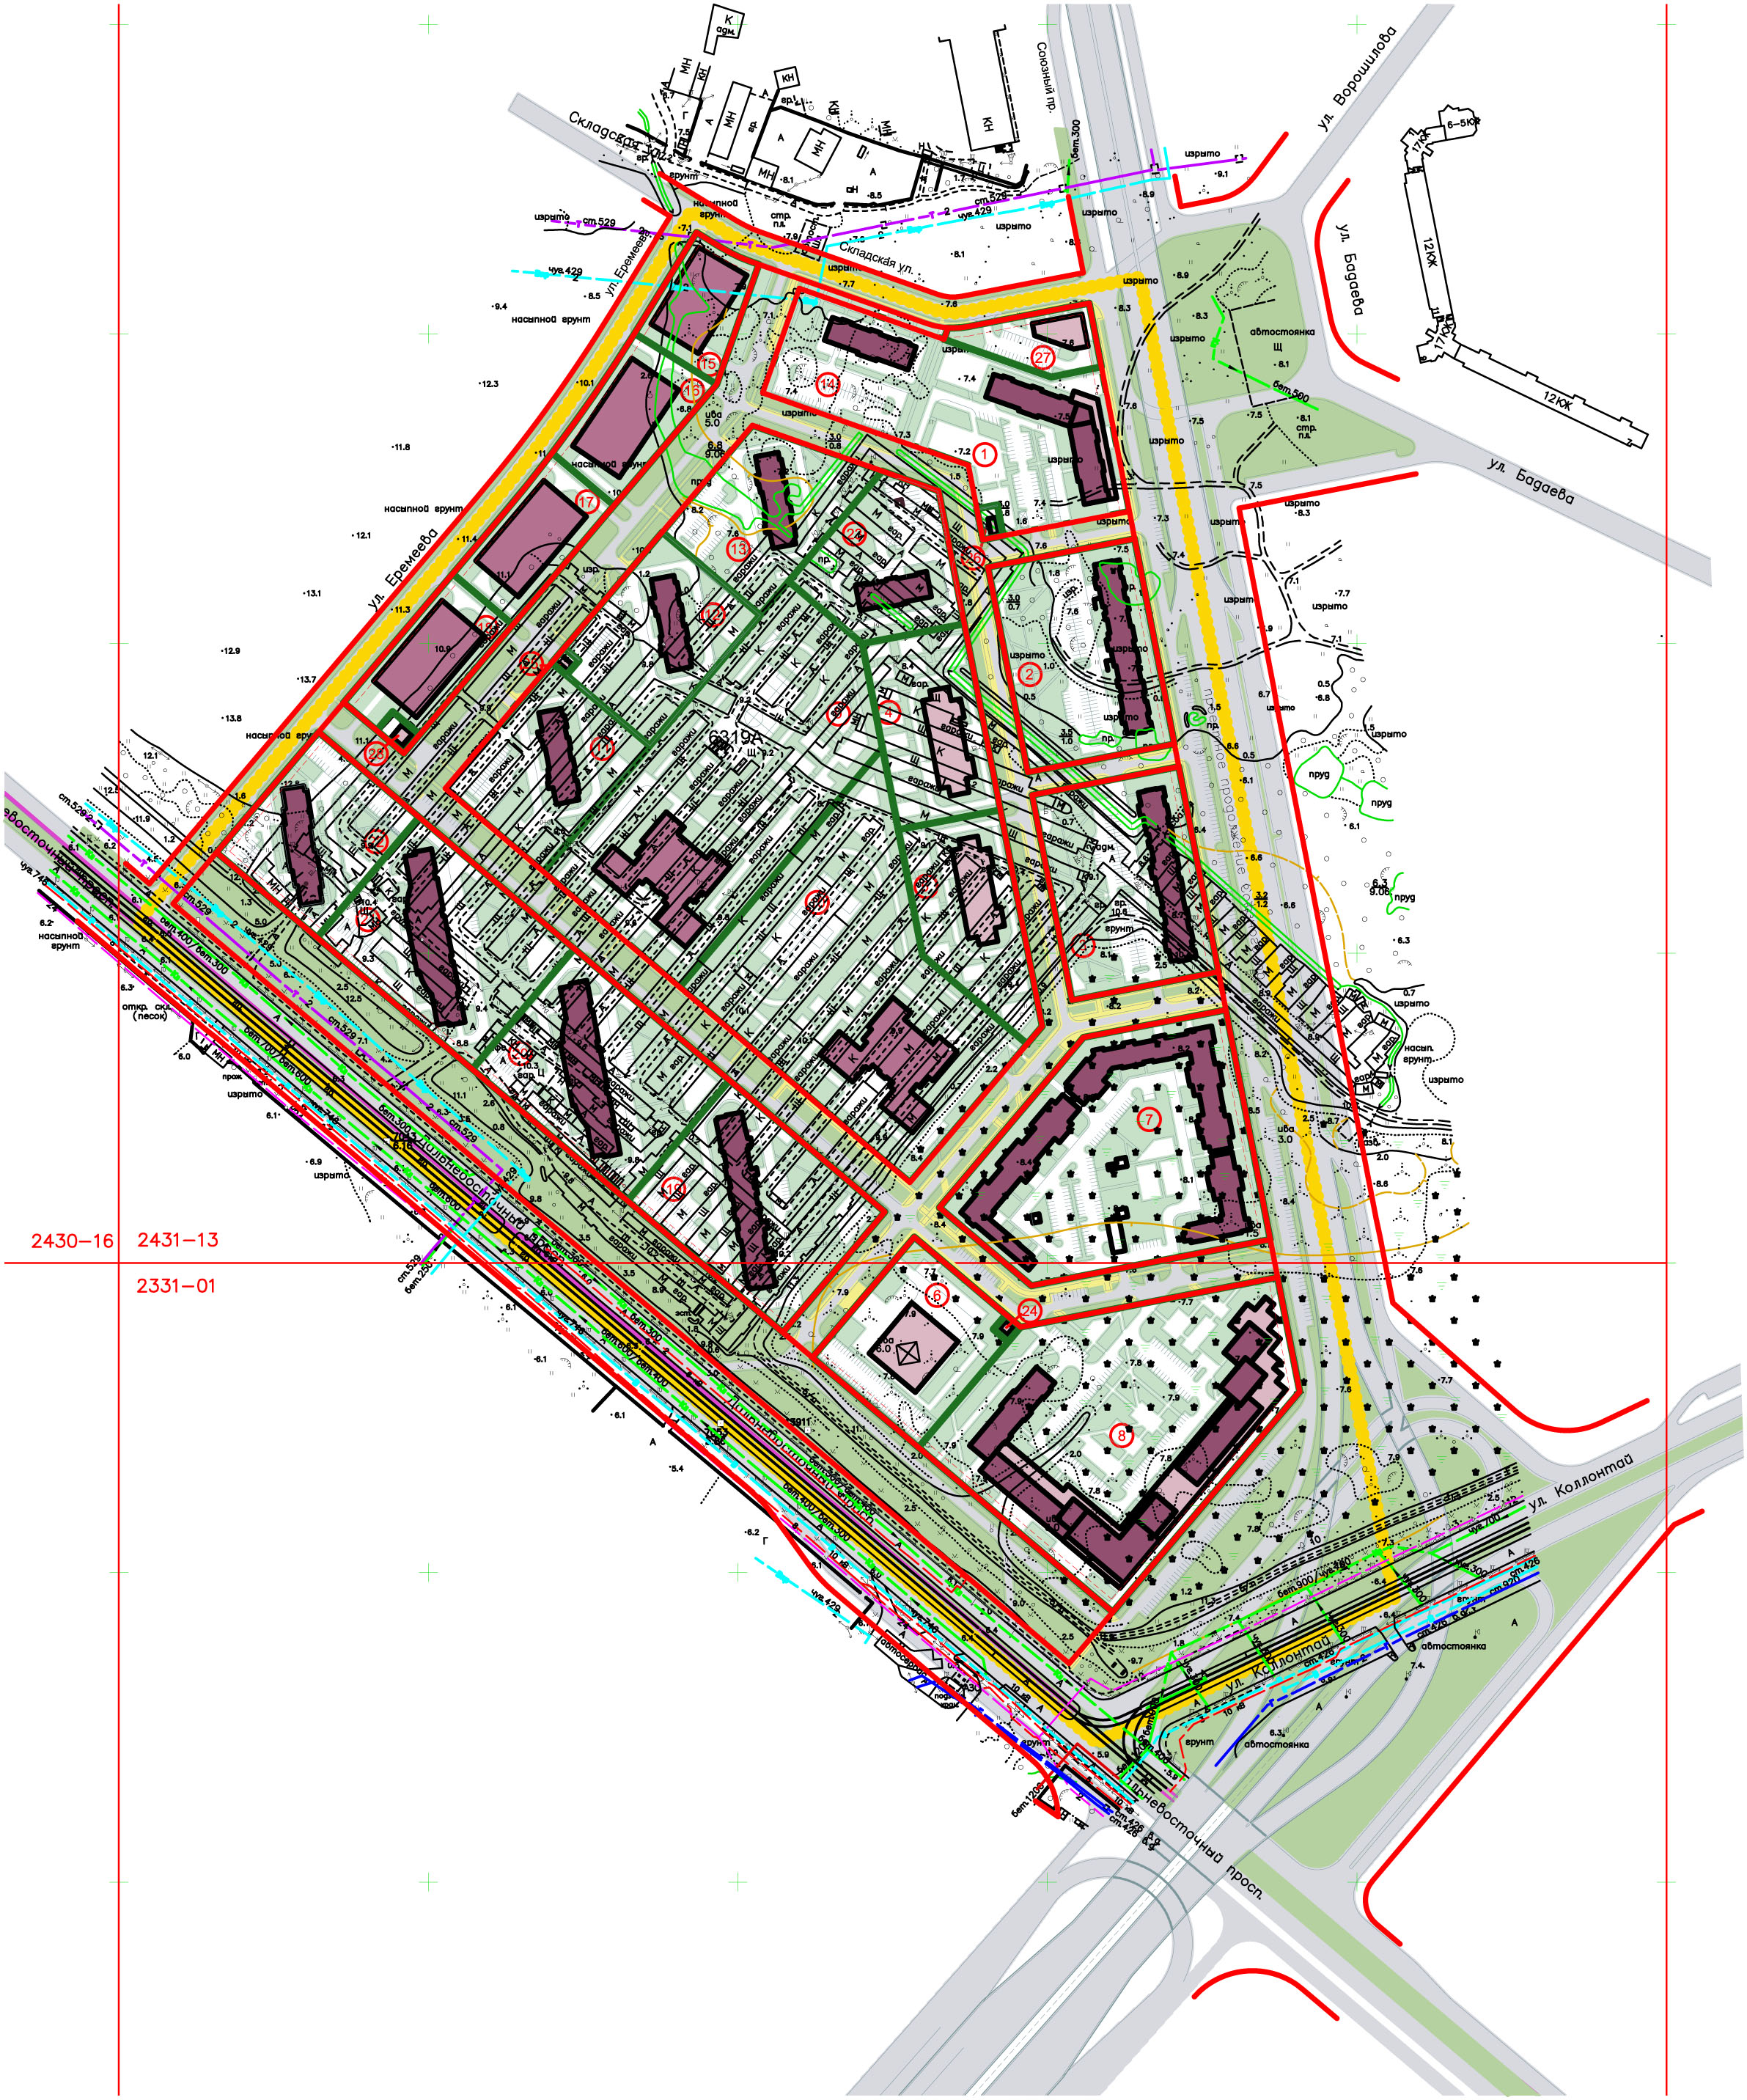
\includegraphics[scale=0.075]{nerd.jpg} 
            \end{center}  
        \end{frame}
        
        \begin{frame}{Машинное обучение}
            Фичи
            \begin{enumerate}
               \item Площадь участка
               \item Максимальная разрешенная высота зданий на участке
               \item Периметр участка
            \end{enumerate}
            Ответы
            \begin{enumerate}
               \item Жилая площадь
               \item Вместимость школ
               \item Вместимость садиков
               \item Число парковочных мест
               \item ...
            \end{enumerate}           
        \end{frame}
        
        \begin{frame}{Майнинг данных}
            \begin{center}
                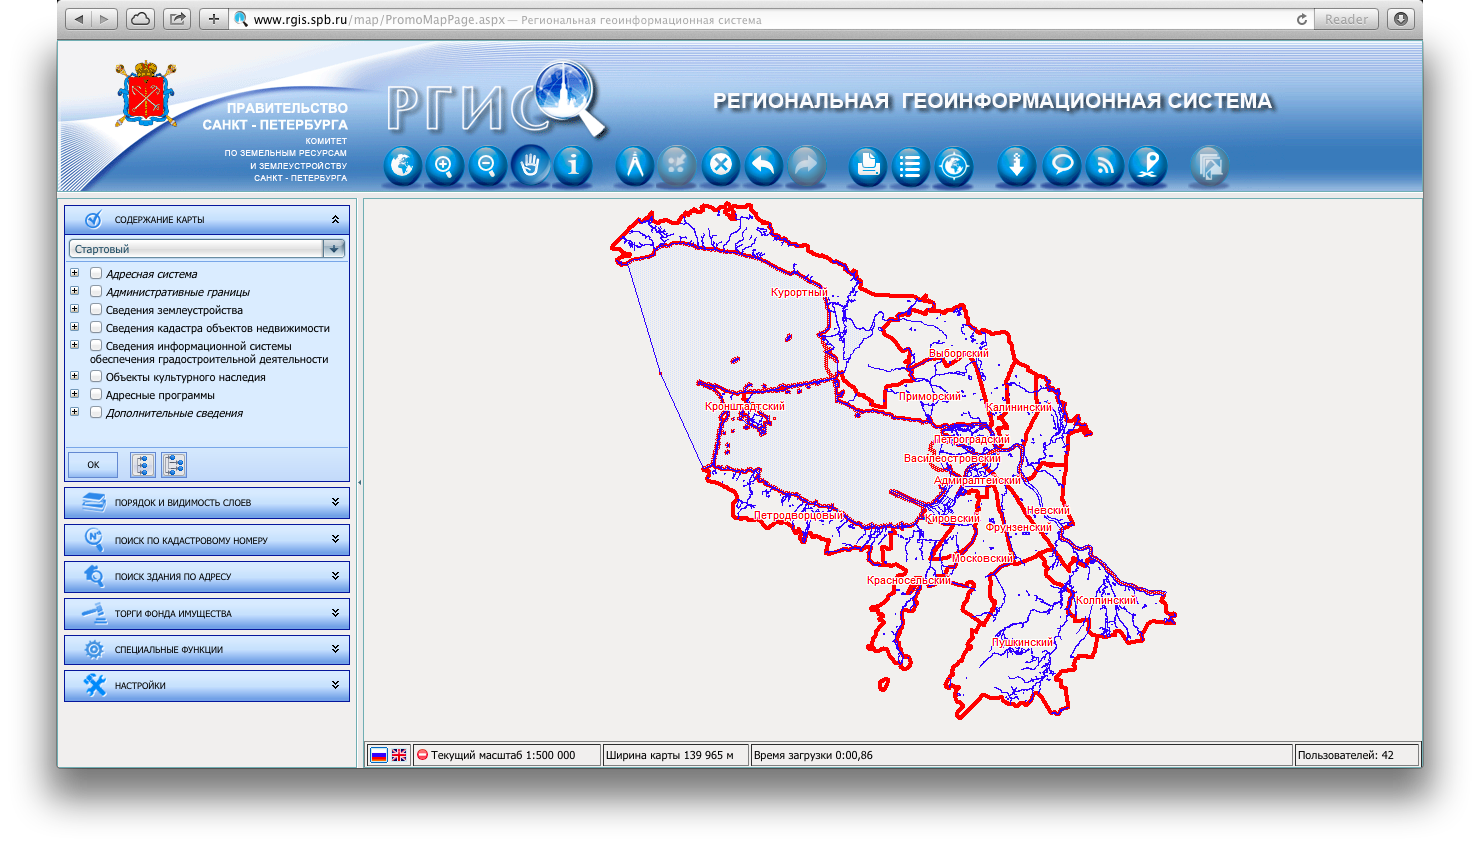
\includegraphics[scale=0.23]{rgis.png}
            \end{center} 
        \end{frame}
        
        \begin{frame}{Майнинг данных}
            \begin{center}
                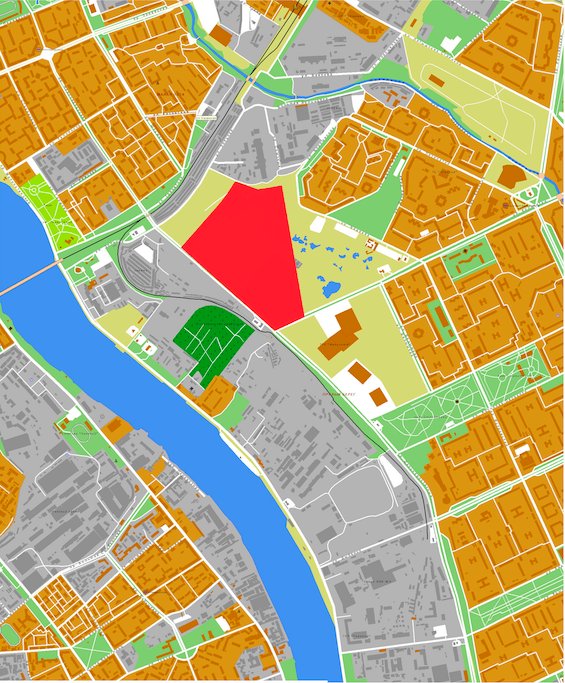
\includegraphics[scale=0.20]{top-plan.png}~
                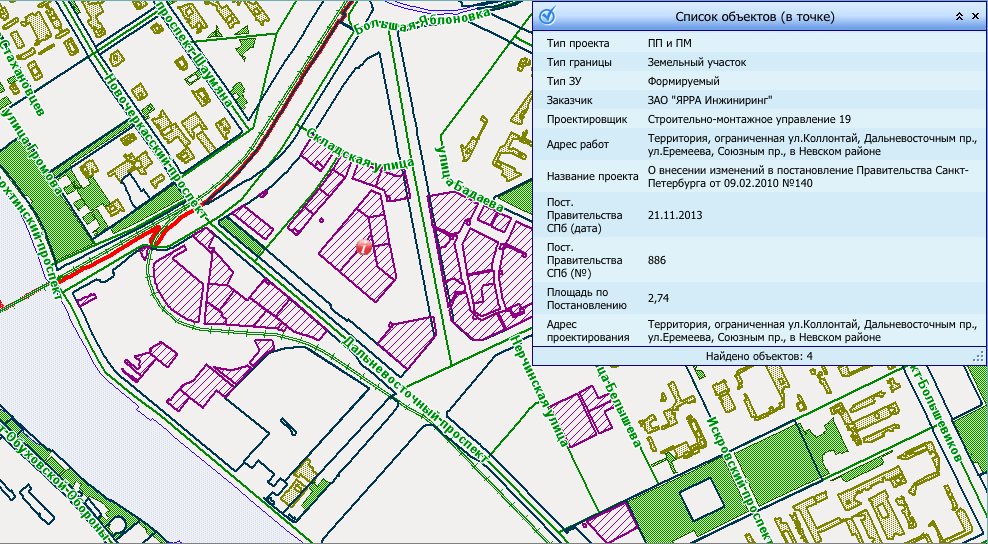
\includegraphics[scale=0.22]{rgis-info.png}
            \end{center} 
        \end{frame}
        
        \begin{frame}{Хорошие данные}
            \begin{center}
                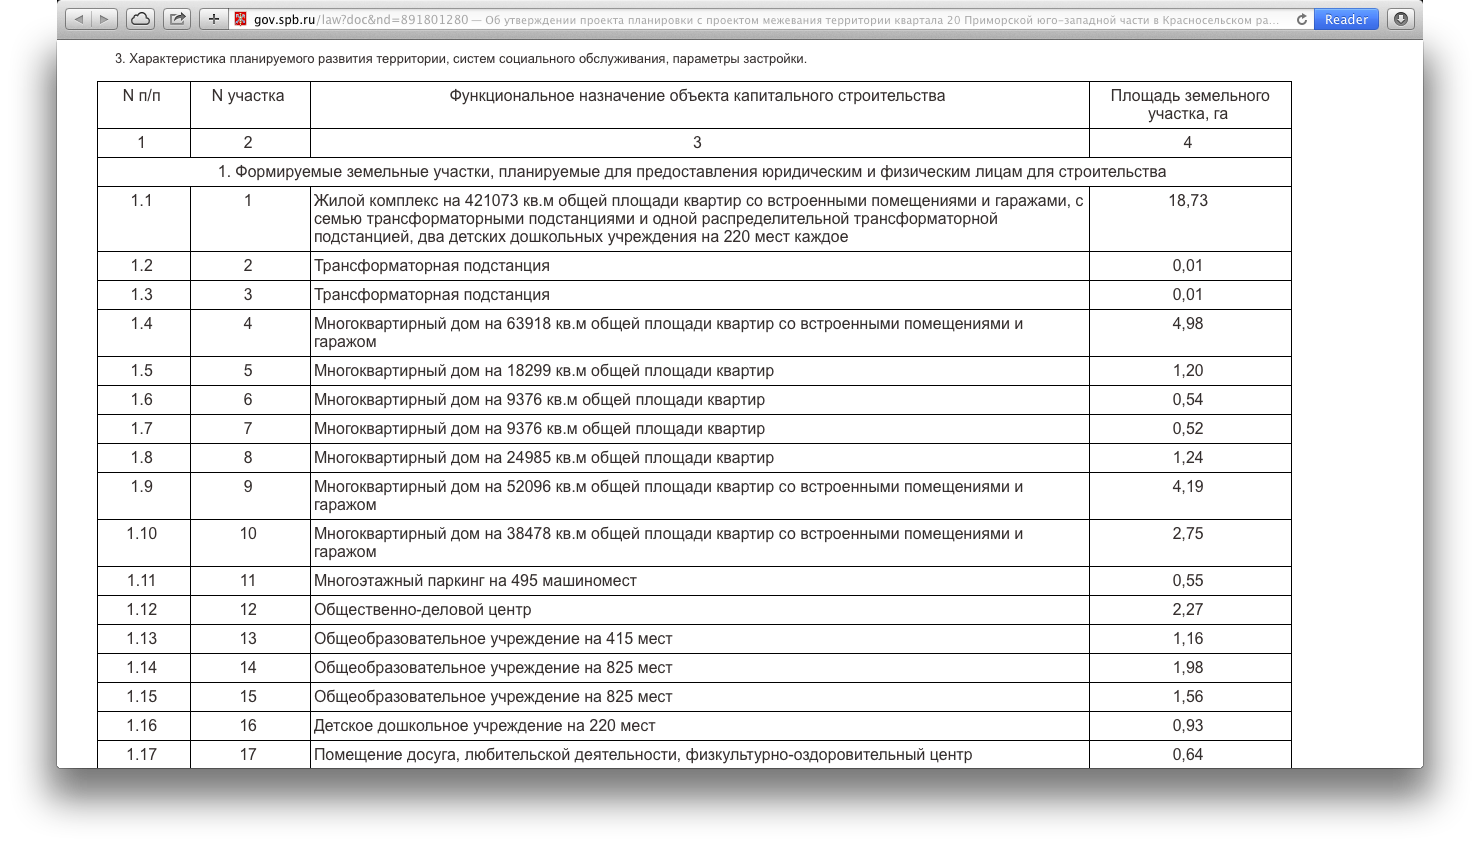
\includegraphics[scale=0.23]{good.png}
            \end{center} 
        \end{frame}      
        
        \begin{frame}{Плохие данные}
            \begin{center}
                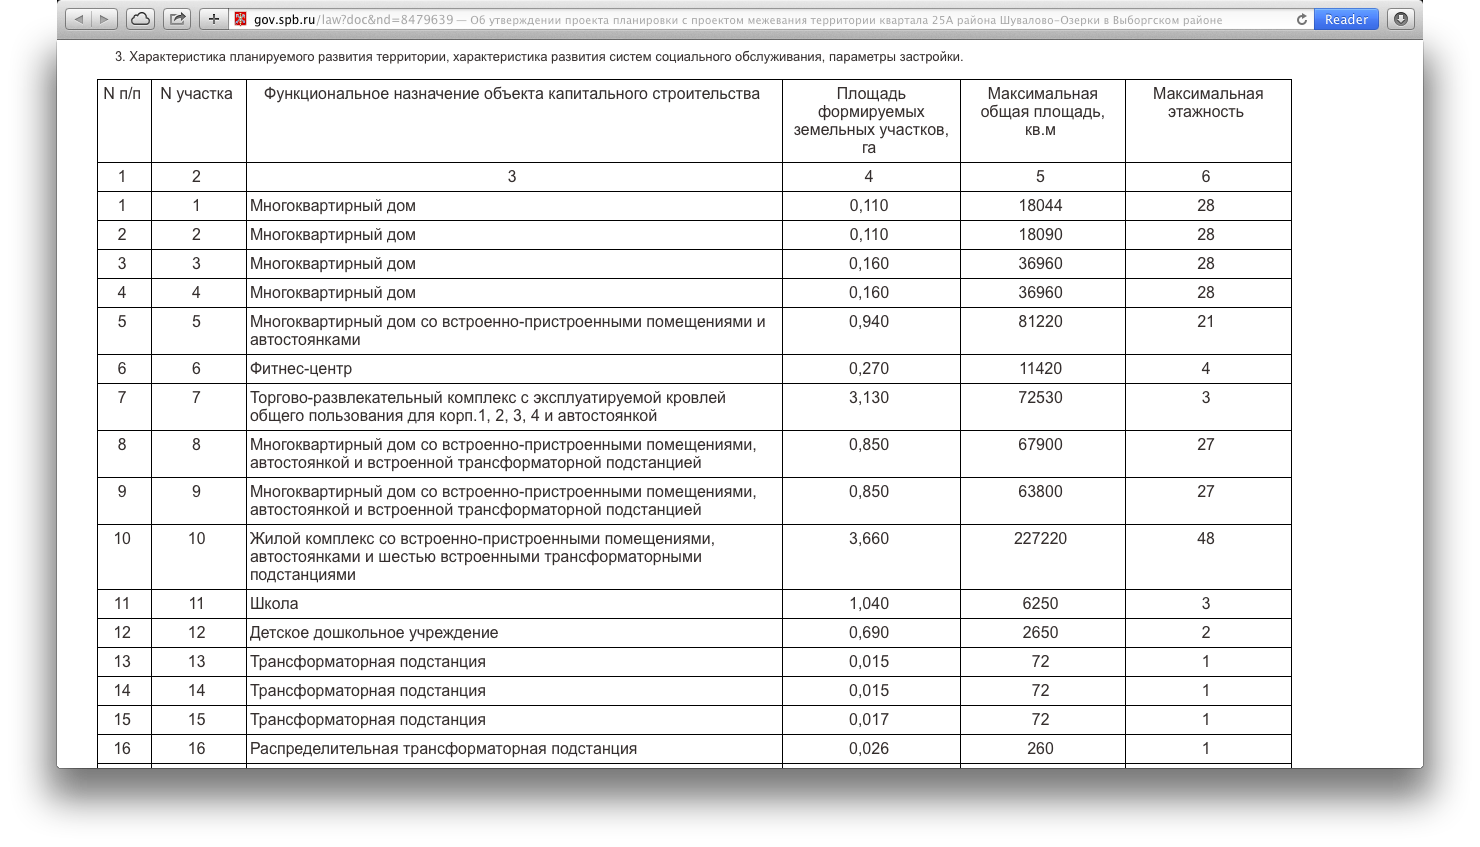
\includegraphics[scale=0.23]{bad.png}
            \end{center} 
        \end{frame}   
        
        \begin{frame}{Итог}
            \begin{center}
                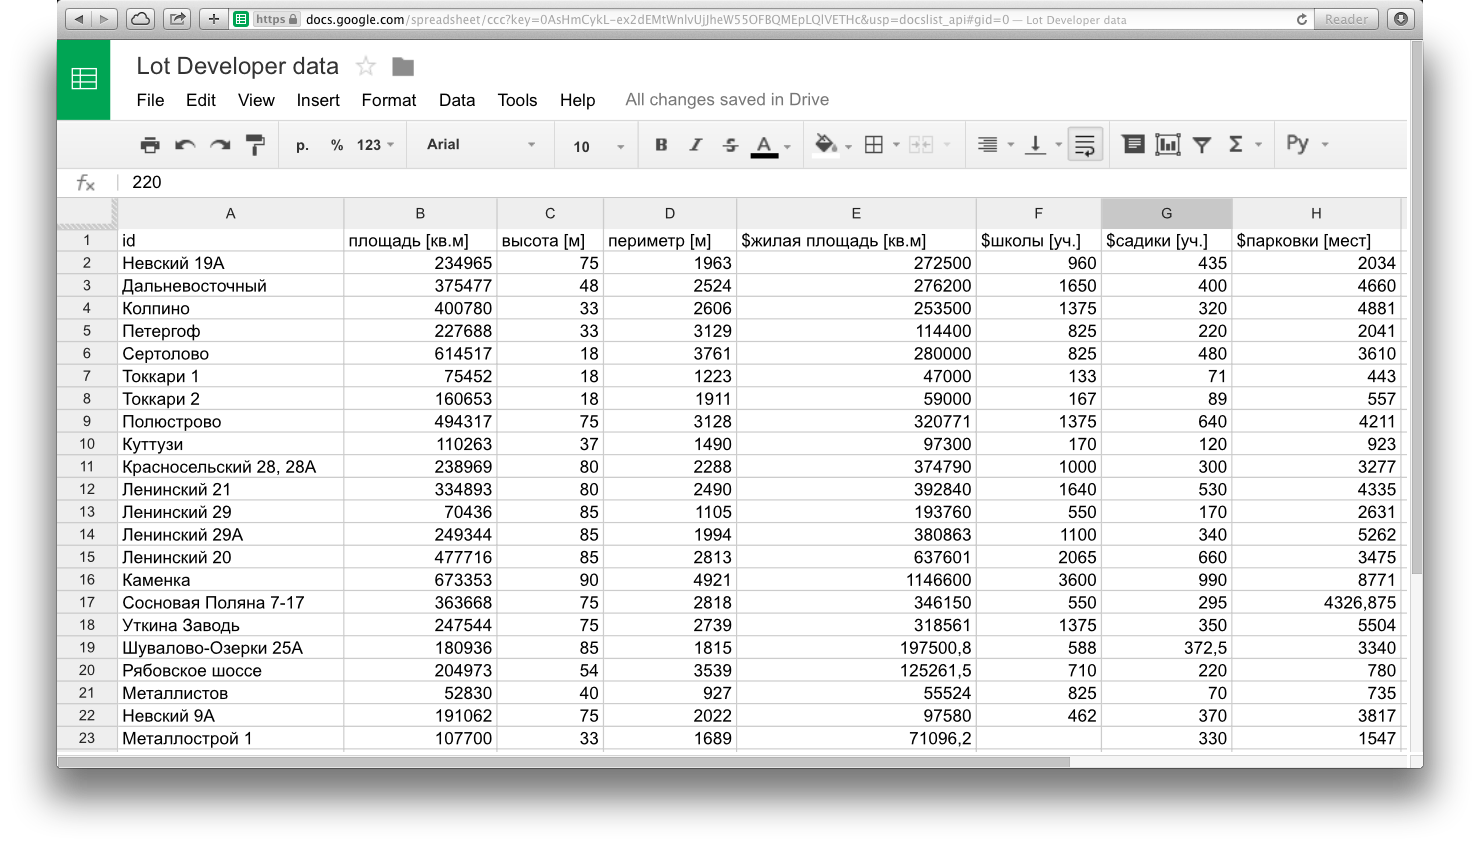
\includegraphics[scale=0.20]{data.png}
                
                30 кварталов по всему Питеру
            \end{center} 
        \end{frame}
        
        
        
        \begin{frame}{Выбор модели}
            \begin{footnotesize}
            
            
            \begin{table} 
		        \begin{tabular} {| c | c | c | c | c |}
				    \hline
				        &    Площадь квартир   &    Парковки    &    Садики    &    Школы   \\
				    \hline
				    Linear Regression    &    67\%    &    67\%    &    86\%    &    71\%    \\		
				    C4.5    &    46\%    &    68\%    &    51\%    &    27\%    \\
				    Perceptron    &    62\%    &    42\%    &   66\%    &    25\%    \\
				    \bf{SVM}    &    \bf{72\%}    &    \bf{78\%}    &   \bf{86\%}    &    \bf{71\%}    \\
				    \hline
			    \end{tabular}
		    \end{table}  
		    
		    
            \end{footnotesize}
        \end{frame}
        
        \begin{frame}{Похожие кварталы}
            \begin{center}
                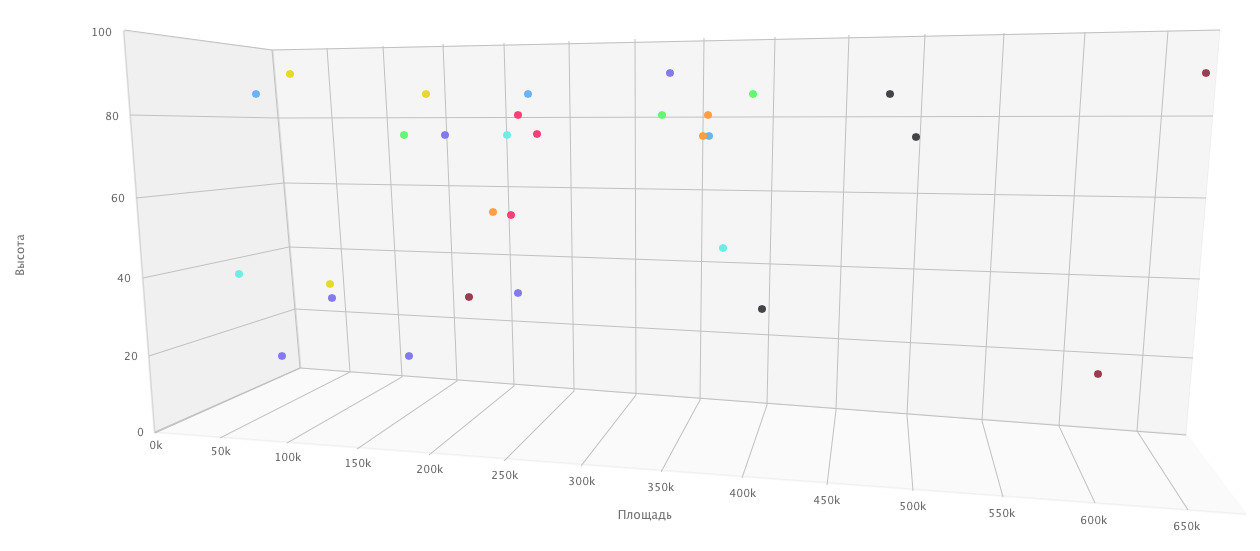
\includegraphics[scale=0.27]{nn.png}
            \end{center}
        \end{frame}
        
        \begin{frame}{Архитектура проекта}
            \begin{center}
                \includegraphics[scale=0.25]{architecture.jpg}
            \end{center}
        \end{frame}
        
        \begin{frame}{Хостинг}
            \begin{center}
                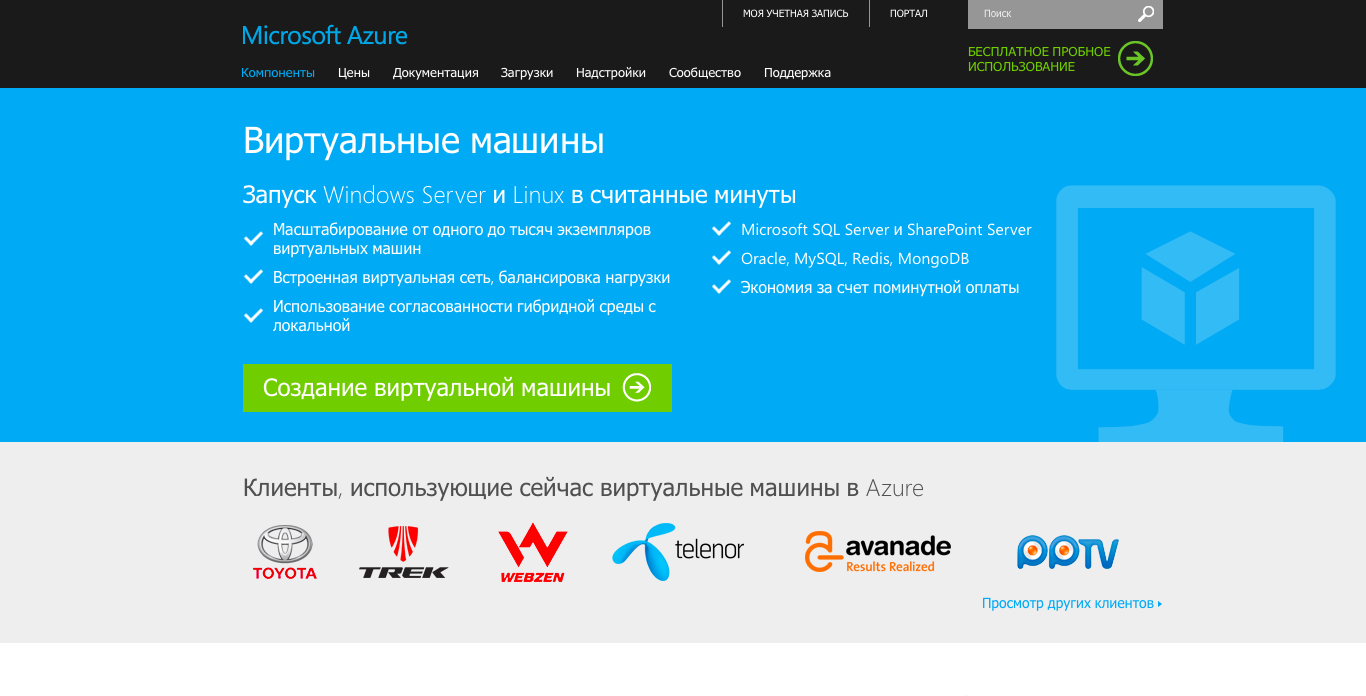
\includegraphics[scale=0.25]{azure.png}
            \end{center}
        \end{frame}
        
        \begin{frame}{В итоге}
            \begin{center}
                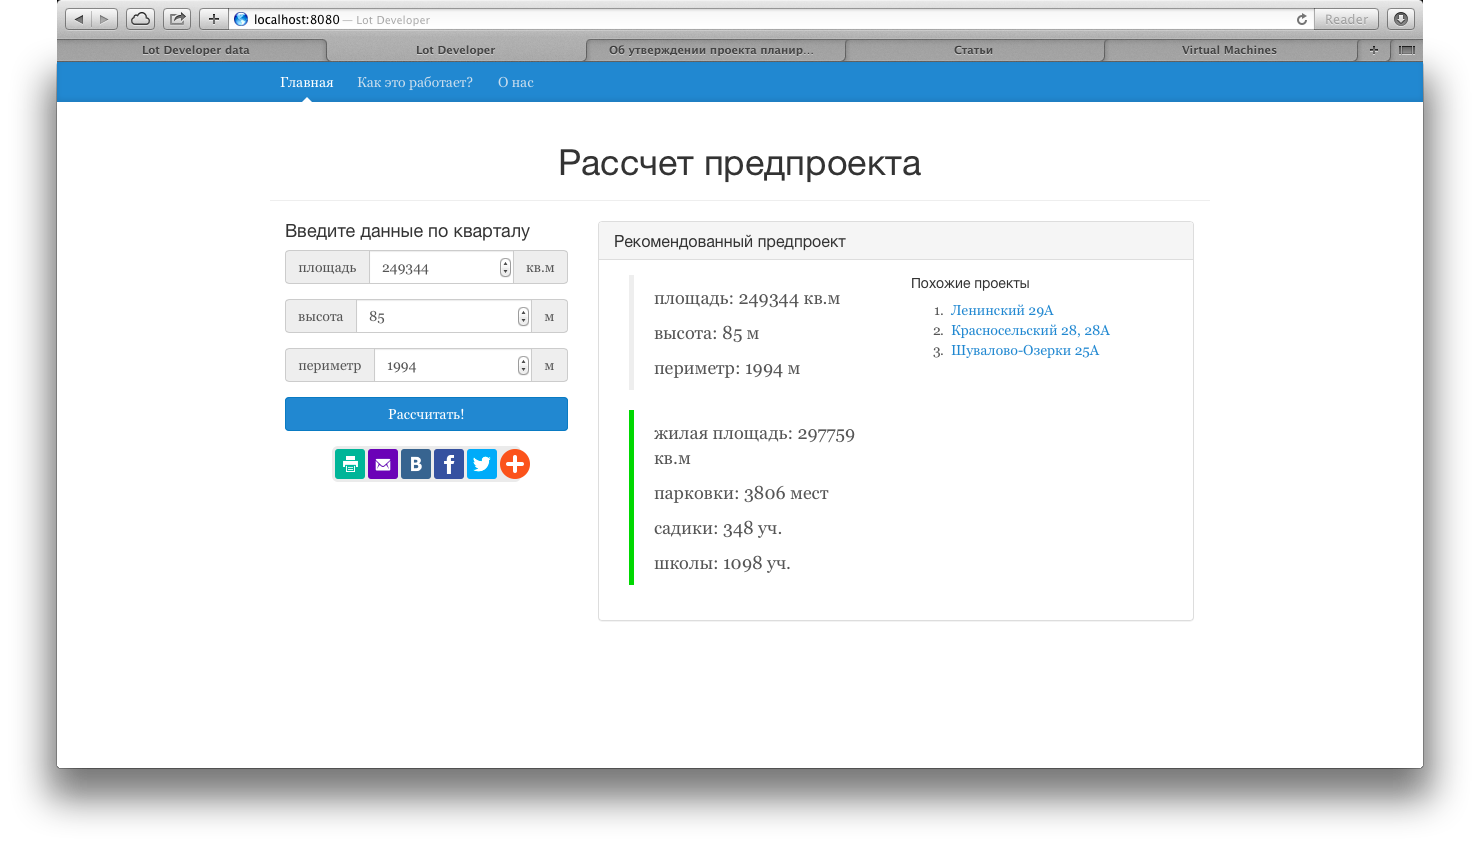
\includegraphics[scale=0.23]{example.png}
            \end{center}
        \end{frame}
        
        \begin{frame}{Используемые технологии}
            \begin{description}
                \item [Сервер]
                    \begin{itemize}
                        \item Java + Spring Framework + Jetty
                        \item Maven
                        \item Spring MVC + JSP
                        \item \bf{Goole Docs API}
                    \end{itemize}
                ~\\
                \item [Клиент]
                    \begin{itemize}
                        \item HTML + CSS + Bootstrap
                        \item JavaScript + jQuery + Ajax
                    \end{itemize}
                ~\\
                \item [Система контроля версий]
                    \begin{itemize}
                        \item Git
                    \end{itemize}
            \end{description}
        \end{frame}
        
        \begin{frame}{Q\&A}
            \begin{center}
                Спасибо за внимание!\\
                \href{http://ciblock.cloudapp.net}{ciblock.cloudapp.net}
            \end{center}
        \end{frame}


\end{document}